%%%%%%%%%%%%%%%%%%%%%%%%%%%%%%%%%%%%%%%%%%%%%%%%%%%%%%%%%%%%%%%%%%%%%%%%%%%
%
% Template for a LaTex article in English.
%
%%%%%%%%%%%%%%%%%%%%%%%%%%%%%%%%%%%%%%%%%%%%%%%%%%%%%%%%%%%%%%%%%%%%%%%%%%%

\documentclass{article}

% AMS packages:
\usepackage{amsmath, amsthm, amsfonts}
\usepackage{algorithm}
\usepackage[hyperref, UTF8]{ctex}
\usepackage[noend]{algpseudocode}
\usepackage{graphicx}
\graphicspath{ {images/} }

% Theorems
%-----------------------------------------------------------------
\newtheorem{thm}{Theorem}[section]
\newtheorem{cor}[thm]{Corollary}
\newtheorem{lem}[thm]{Lemma}
\newtheorem{prop}[thm]{Proposition}
\theoremstyle{definition}
\newtheorem{defn}[thm]{Definition}
\theoremstyle{remark}
\newtheorem{rem}[thm]{Remark}

\makeatletter
\def\BState{\State\hskip-\ALG@thistlm}
\makeatother
%\newcommand*{\rom}[1]{\expandafter\@slowromancap\romannumeral #1@}
\newcommand{\rom}[1]{\uppercase\expandafter{\romannumeral #1\relax}}
% Shortcuts.
% One can define new commands to shorten frequently used
% constructions. As an example, this defines the R and Z used
% for the real and integer numbers.
%-----------------------------------------------------------------
\def\RR{\mathbb{R}}
\def\ZZ{\mathbb{Z}}

% Similarly, one can define commands that take arguments. In this
% example we define a command for the absolute value.
% -----------------------------------------------------------------
\newcommand{\abs}[1]{\left\vert#1\right\vert}

% Operators
% New operators must defined as such to have them typeset
% correctly. As an example we define the Jacobian:
% -----------------------------------------------------------------
\DeclareMathOperator{\Jac}{Jac}

%-----------------------------------------------------------------
\title{Report of paper Isotopic Approximation within a Tolerance Volume}
\author{ShengweiZHANG\\
  %% \small Dept. Templates and Editors\\
  %% \small E12345\\
  %% \small Spain
}

\begin{document}
\maketitle

%% \abstract{Compiling Embedded\_thin\_shell progress}
\section{Target}
For a surface $\mathbb{S}$, we construct a tolerance volume $\Omega$ which is a topological thickening of a surface $\mathbb{S}$. Our goal is to generate as output a surface triangle mesh located within $\Omega$, isotopic to the boundary components of $\Omega$, and with a low triangle count.
\section{Algorithm Overview}
Input: a $\sigma$-dense set $\mathtt{S}$ sampled on the tolerance boundary $\partial \Omega$.\par
Main Steps:
\begin{description}
  \item[1] Refine, select points from $\partial \Omega$ to construct $\Gamma$ -- a approximation of volume $\Omega$, By adding points to the triangulation $\tau$, and maintaining a piecewise-linear function interpolated on the triangulation.
  \item[2] Simplification, Simplify the zero point set $\mathcal{Z}$ of the piecewise-linear function(the final output), By do on $\tau$ edge collapse in $\partial \Gamma$, perform mutual tessellation between $\mathcal{Z}$ and $\partial \Gamma$, then do edge collapse of all edges again.
\end{description}

\section{Construct the $\Omega$ from a input Surface $\mathbb{S}$}
TODO
\section{Refinement}
\subsection{Initialization}
Construct an initial 3D Delaunay triangulation ($\tau$) with the eight corners of a loose bounding box of $\mathtt{S}$,  and maintaining a piecewise-linear function $f(\mathtt{s})$ interpolated on the triangulation, and the error function $\epsilon(\mathtt{s})$:
\begin{equation}
  \begin{array}{l}
f(\mathtt{s}) \approx \left\{
\begin{array}{lcl}
{+1} &\text{if} & s \in \partial \Omega_1 \text{ outer boundary} \\
{-1} &\text{if} & s \in \partial \Omega_2 \text{ inner boundary} \\  
\end{array}  
\right.\\
\epsilon(\mathtt{s}) \approx \left\{
\begin{array}{lcl}
{\parallel f(\mathtt{s})-1 \parallel} &\text{if} & s \in \partial \Omega_1 \text{ outer boundary} \\
{\parallel f(\mathtt{s})+1 \parallel} &\text{if} & s \in \partial \Omega_2 \text{ inner boundary} \\  
\end{array}  
\right.\\
\end{array}
\end{equation}
Here we define midpoints on the edges between $\partial \Omega_1$ and $\partial \Omega_2$, as zero-points $\mathcal{Z}$.
\subsection{Procedure}
Our goal is to construct a $\Gamma$ approximate $\Omega$. We get it by insert one sample point at a time into $\tau$ and update the Delaunay property, until $\mathcal{Z}$ classifies all samples of  $\mathtt{S}$ as good, or equivalently, until $\mathcal{Z}$ separates the boundaries $\partial \Omega_i$ of $\Omega$.
Greedy adding the sample point in  $\mathtt{S}$ withing the maximum error, until $\epsilon(\mathtt{s})<1$ is a natural idea, unfortunately, its not enough for two reasons:
\begin{itemize}
\item First as we use a finite sample of $\partial \Omega$, even if all sample points end up being well classified, this still leaves the possibility that $\mathcal{Z}$ crosses $\partial \Omega$ in-between the samples.
 \item Second the normal directions maybe grossly wrong even in locally smooth areas.
 \end{itemize}
So our solution is:
\begin{description}
 \item[1] Adding the sample point in  $\mathtt{S}$ withing the maximum error, until $\epsilon(\mathtt{s}) < 1- \alpha$.
 \item[2] Adding the sample point nearest to the circumcenter of a bad tetrahedron.
\end{description}
\par To solve the first problem, we enforce the constraint let $f(\mathtt{s}) < 1 - \alpha$, and add an upper bound of $\alpha / \sigma$ on the Lipschitz constant of the piecewise-linear function to ensure that the zero-set does not cross $\partial \Omega$.  Noticing that  the Lipschitz constant $c=2/h$, so $2/h < \alpha / \sigma$, and a tetrahedron between $\partial \Omega_1$ and $\partial \Omega_2$ with $h \le 2\sigma / \alpha$ is a bad tetrahedron. $\alpha$ is set to 0.2.
\par To solve the second problem, the piecewise-linear function defined by each tetrahedron $\mathtt{t}$ classifies well the samples of  $\mathtt{S}$ on both the points of $\partial \Omega$. But can't classifiy the sample points in $\partial \Omega$ that are nearest to the vertices of a shrunk copy of $\mathtt{t}$, then $\mathtt{t}$ is a bad tetrahedron. The size of this shrunk copy is set to 0.7.
\section{Simplification}
\subsection{Overview}
In this step our goal is to reduce the complexity of the zero-set $\mathcal{Z}$ via the decimation of $\tau$. We peform the decimation by flowing steps:
\begin{description}
  \item[1.] Collapse edges of $\partial \Gamma$.
  \item[2.] Mutualtessllation of $\mathcal{Z}$ into $\tau$.
  \item[3.] Collapse edges of $\mathcal{Z}$.
  \item[4.] Collapse all possibile edges.
\end{description}
\subsection{collapse edges of $\partial \Gamma$}
Define the an edge PQ collapse into a target point $\mathtt{T}$, We have conditions as flows:
\begin{itemize}
  \item Keep a valid triangulation $\tau$. (common condition)
  \item Kernel area $K_{\tau}(PQ)$ of one ring edge PQ is not empty, as T must locate into that area. (common condition)
  \item Keep $\epsilon(s) < 1-\alpha$.
\end{itemize}

\subsection{Mutualtessllation of $\mathcal{Z}$ into $\tau$}
TODO
\subsection{Collapse edges of $\mathcal{Z}$}
With to common condition as above, and a different third condition: after edge collapse, the zero-set surface can't corss $\partial \Omega$.
\subsection{Collapse all possibile edges}
In fact in this step we perform edge collapse between $\partial \Gamma$ and $\mathcal{Z}$, under the two common conditions. Collapsing an edge between a vertex of $\Gamma$ and a vertex of $\mathcal{Z}$ tends to increase the area of the one-ring of PQ  and hence increases the probability that an edge of $\mathcal{Z}$ is collapsible.
%% \begin{figure}[H]
%% 	\onecolumn
%% 	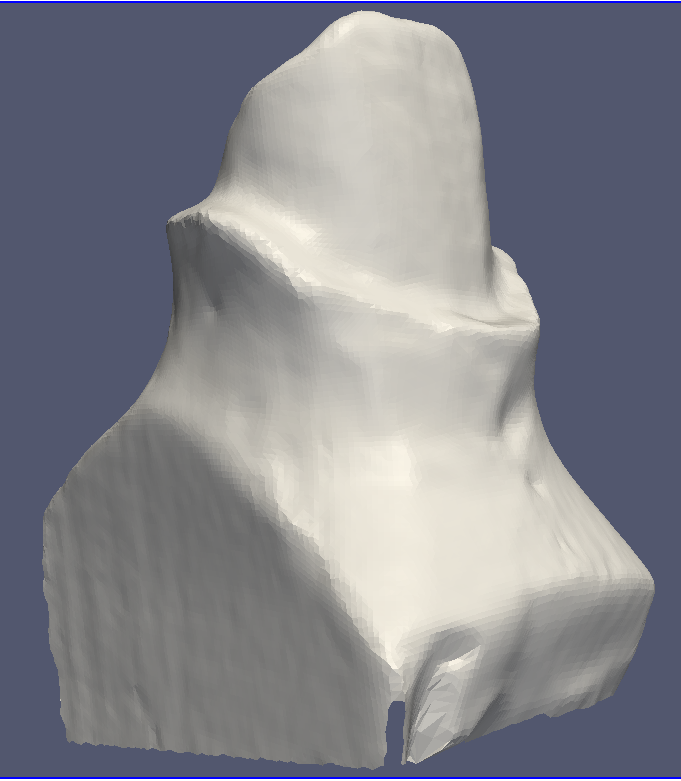
\includegraphics[width=6cm]{our_basic}
%% 	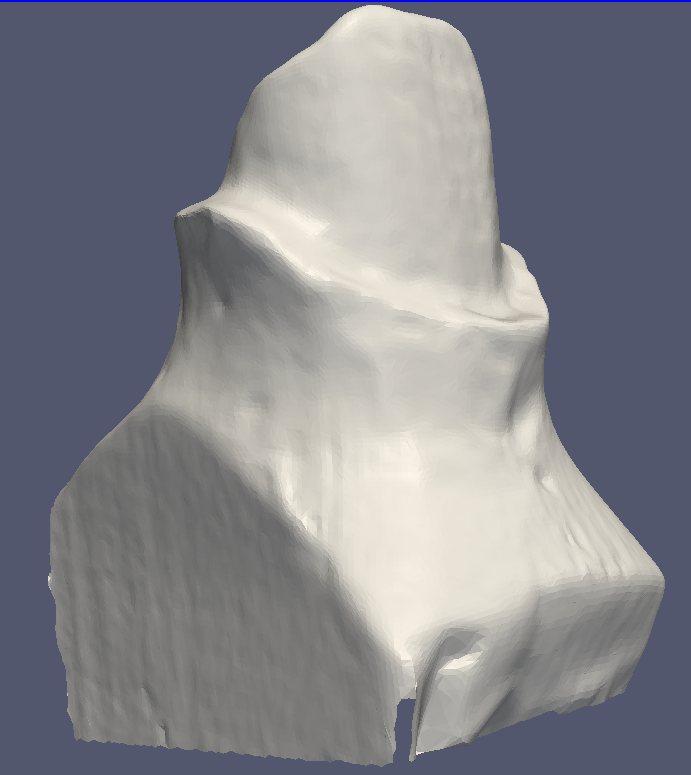
\includegraphics[width=6cm]{smooth_0}
%% 	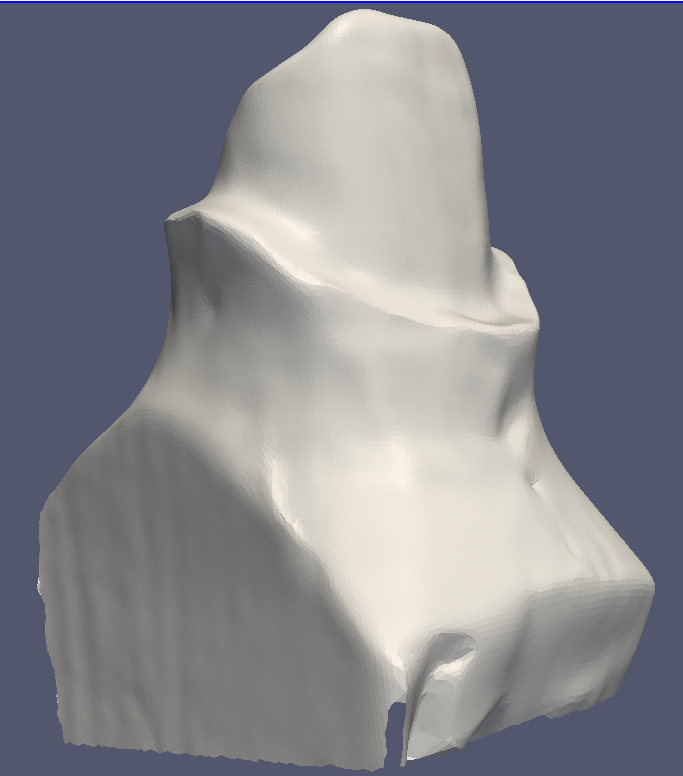
\includegraphics[width=6cm]{smooth_1}
%% 	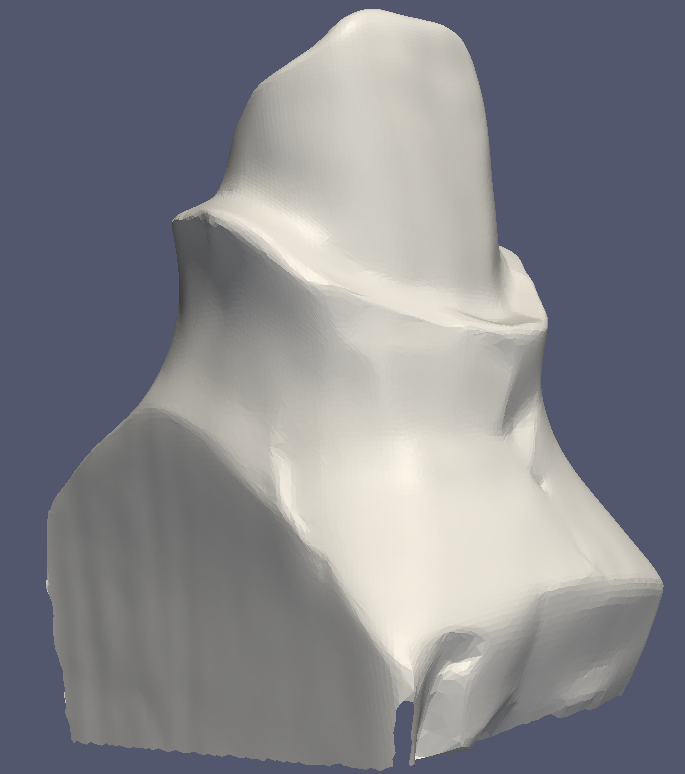
\includegraphics[width=6cm]{smooth_2}
%% 	\caption[效果对比]
%% 	{Atos不同程度光顺与标准双边滤波(3次迭代,边的一环邻域)效果对比,左上角为标准双边滤波效果,另外为geo inspect取不同滤波半径的结果,滤波半径依次扩大.}
%% 	\centering
%% \end{figure}

\end{document}
